\documentclass[runningheads]{llncs}
\usepackage{amsmath}
\usepackage{amsfonts}
\usepackage{amssymb}
\usepackage{verbatim}
\usepackage[pdftex]{graphicx}
  \graphicspath{{./pics/}}
  \DeclareGraphicsExtensions{.pdf}
\usepackage{tikz}
\usetikzlibrary{arrows,automata,shapes}
\usetikzlibrary{positioning}
  
\overfullrule 5pt
\widowpenalty=10000
\clubpenalty =10000
\interlinepenalty=10

\newcommand{\eps}{\varepsilon}
\newcommand{\R}{}
\newcommand{\J}{}
\newcommand{\makeset}[2]{\ensuremath{ \{ #1 \: | \: #2 \} }}
\renewcommand{\sc}{\mathrm{sc}}

\spnewtheorem{fact}{Fact}{\bf}{\it}

\newcommand{\boxcomment}[1]{\begin{center}\fbox{\parbox{.9\linewidth}{#1}}\end{center}}
\newcommand{\tomas}[1]{\boxcomment{{\bf Tomas:} #1}}
\newcommand{\galina}[1]{\boxcomment{{\bf Galina:} #1}}



\begin{document}
\title{On the State Complexity of the Reverse of \R-~and \J-trivial Regular Languages}
\titlerunning{State Complexity of the Reverse of \R- and \J-trivial Regular Languages}
\authorrunning{G. Jir\'{a}skov\'{a}, T. Masopust}
\author{
  Galina Jir\'{a}skov\'{a}\,\inst{1,}\thanks{Research supported by VEGA grant 2/0183/11 and by grant APVV-0035-10.}
  \and
  Tom\'{a}\v{s} Masopust\,\inst{2,3,}\thanks{Research supported by GA{\v C}R grant P202/11/P028 and by RVO: 67985840.}}
\institute{
  Mathematical Institute, Slovak Academy of Sciences\\
  Gre{\v s}{\' a}kova 6, 040 01 Ko\v{s}ice, Slovak Republic\\
  \email{jiraskov@saske.sk}
  \and
  Institute of Mathematics, Academy of Sciences of the Czech Republic\\
  {\v Z}i{\v z}kova 22, 616 62 Brno, Czech Republic\\
  \email{masopust@math.cas.cz}
  \and
  Institute for Computer Science, University of Bayreuth
}

\maketitle
\begin{abstract}
  The tight upper bound on the state complexity of the reverse of \R-trivial and \J-trivial regular languages of the state complexity  is . The witness is ternary for \R-trivial regular languages and -ary for \J-trivial regular languages. In this paper, we prove that the bound can be met neither by a binary \R-trivial regular language nor by a \J-trivial regular language over an -element alphabet. We provide a characterization of tight bounds for \R-trivial regular languages depending on the state complexity of the language and the size of its alphabet. We show the tight bound for \J-trivial regular languages over an -element alphabet and a few tight bounds for binary \J-trivial regular languages. The case of \J-trivial regular languages over an -element alphabet, for , is open.
\end{abstract}

\section{Introduction}
  Regular languages of simple forms play an important role in mathematics and computer science. The reader is referred to, e.g.,~\cite{Bojanczyk:2012,2013arXiv1303.0966C,Rogers:2007} for a few applications of \J-trivial (piecewise testable) languages. The aim of this paper is to investigate the state complexity of the reverse of two such language classes, namely of \R-trivial and \J-trivial regular languages. 
  
  For a regular language, the state complexity is the number of states of its minimal automaton representation. The reverse of an automaton or of a language is a classical operation whose state complexity is exponential in the worst case. There exist binary witness languages of the state complexity  with the reverse of the state complexity , see~\cite{le81,yzs94}. This even holds true for union-free regular languages defined by regular expressions without the union operation~\cite{ijfcsJiraskovaM11}.

  As mentioned above, we consider languages defined by Green's equivalence relations, namely \R-trivial and \J-trivial regular languages. Let  be a monoid and  and  be two elements of . Green's relations , \R, \J, and  on  are defined so that
     if and only if ,
     if and only if ,
     if and only if , and
    .
  For ,  is \mbox{-}trivial if  implies , for all  in . A language is {\em \mbox{-}trivial} if its syntactic monoid is -trivial. Note that -trivial regular languages coincide with {\em star-free} languages~\cite[Chapter~11]{lawson2003finite} and that -trivial, \R-trivial and \J-trivial regular languages are all star-free. Moreover, \J-trivial regular languages are both -trivial and \R-trivial.

  Equivalently, a regular language is \R-trivial if and only if it is a finite union of languages of the form , where , , and , or if and only if it is accepted by a partially ordered minimal DFA~\cite{BrzozowskiF80}. Similarly, a regular language is \J-trivial (or {\em piecewise testable}) if and only if it is a finite boolean combination of languages of the form , where  and , or if and only if the minimal DFAs for both the language and the reverse of the language are partially ordered~\cite{Simon1972,Simon1975}. Other automata representations of these languages can be found, e.g., in~\cite{LauserCIAA} and the literature therein. Stern~\cite{Stern85a} suggested a polynomial algorithm 
  of order  in the number of states and transitions of the minimal DFA 
  to decide whether a regular language is \J-trivial. Trahtman~\cite{Trahtman2001} recently improved this result to a quadratic algorithm. 
  
  In~\cite{ciaa2012}, we have shown that the upper bound on the state complexity of the reverse of \R-trivial and \J-trivial regular languages is  for languages of the state complexity . We have also shown that this bound can be met by a ternary \R-trivial regular language and conjectured that an ()-element alphabet is sufficient for \J-trivial regular languages of the state complexity  to meet the upper bound, which was later proved in~\cite{BrArXiv12}. In this paper, we prove the optimality of the size of these alphabets. Namely, we prove that the bound on the state complexity of the reverse can be met neither by a binary \R-trivial regular language (Lemma~\ref{lem:binaryRtriv_upper}) nor by a \J-trivial regular language over an -element alphabet (Theorem~\ref{thm:boundJtriv}). As a result, we provide a complete characterization of tight upper bounds for \R-trivial regular languages depending on the state complexity of the language and the size of its alphabet (Theorem~\ref{thm1}). Finally, we prove a tight upper bound for \J-trivial regular languages over -element alphabets (Theorem~\ref{thm3}) and several tight bounds for binary \J-trivial regular languages (Table~\ref{tab}). The case of \J-trivial regular languages over -element alphabets, for , is left open.
  

\section{Preliminaries and Definitions}
  We assume that the reader is familiar with automata and formal language theory. The cardinality of a set  is denoted by , and the powerset of  is denoted by . An alphabet is a finite nonempty set. The free monoid generated by an alphabet  is denoted by . A string over  is any element of , and the empty string is denoted by .

  A {\em nondeterministic finite automaton\/} (NFA) is a 5-tuple , where  is the finite nonempty set of states,  is the input alphabet,  is the set of initial states,  is the set of accepting states, and  is the transition function that can be extended to the domain . The language {\em accepted\/} by  is the set . The NFA  is {\em deterministic\/} (DFA) if  and  for every  in  and  in . In this case we identify singleton sets with their elements and simply write  instead of . Moreover, the transition function  is a total map from  to  that can be extended to the domain . Two states of a DFA are {\em distinguishable\/} if there exists a string  that is accepted from one of them and rejected from the other; otherwise they are {\em equivalent}. A DFA is {\em minimal\/} if all its states are reachable and pairwise distinguishable. A non-accepting state  such that , for all  in , is called a {\em dead\/} state.
  
  The \emph{state complexity} of a regular language , denoted by , is the number of states in the minimal DFA accepting the language .

  The {\em subset automaton\/} of an NFA  is the DFA   constructed by the standard subset construction.
  
  Let  be a DFA. The reachability relation  on the states of  is defined by  if there exists a string  in  such that . The DFA  is {\em partially ordered\/} if the reachability relation  is a partial order. For two states  and  of , we write  if  and . A state  is {\em maximal\/} if there is no state  such that . 

  The \emph{reverse  of a string \/} is defined by  and , for  in  and  in . The \emph{reverse of a language\/}  is the language . The \emph{reverse of a DFA\/}  is the NFA  obtained from  by reversing all transitions and swapping the role of initial and accepting states. 
  The following result says that there are no equivalent states in the subset automaton of the reverse of a minimal DFA. We use this fact in the paper when proving the tightness of upper bounds. By this fact, it is sufficient to show that the corresponding number of states is reachable in the subset automaton since the distinguishability always holds.
  \begin{fact}[\cite{br63}]\label{le:equiv}
    All states of the subset automaton corresponding to  the reverse of a minimal DFA are pairwise distinguishable.
    \qed
  \end{fact}

  In what follows we implicitly use the characterization that a regular language is \R-trivial if and only if it is accepted by a minimal partially ordered DFA and that it is \J-trivial if and only if both the language and its reverse are accepted by minimal partially ordered DFAs. This characterization immediately implies that \J-trivial regular languages are closed under reverse. However, \R-trivial regular languages are not closed under reverse since not all \R-trivial regular languages are \J-trivial. For instance, the \R-trivial regular language of Fig.~\ref{fi:binaryRtriv} is not \J-trivial, hence the minimal DFA for its reverse is not partially ordered.

  The following lemma shows that in some cases we do not need to distinguish between DFAs with and without dead state. In particular, we can get a result for DFAs without a dead state immediately from the analogous result for DFAs with a dead state or vice versa.\footnote{We are grateful to an anonymous referee for pointing out this observation.} 
  \begin{lemma}\label{lem:complement}
    Let  be a regular language. Then , where  denotes the complement of . 
    In particular, we have .
  \end{lemma}
\begin{proof}
    Let  be a minimal DFA accepting . Then  constructed from  by swapping accepting and non-accepting states is a minimal DFA accepting . The second part now follows by the observation that . 
    Indeed,  if and only if  if and only if  if and only if  if and only if .
    \qed
  \end{proof}


  Let  be a DFA with a dead state reaching the upper bound on the reverse. This lemma says that if the complement of  does not have a dead state, the same result can be reached by DFAs without a dead state. Indeed, the complement of  reaches the bound. However, Table~\ref{tab} demonstrates that there are cases where this technique fails because both the DFA and its complement have a dead state. 
  
  Immediate consequences of this lemma combined with the known results are formulated below.
  \begin{corollary}\label{cor:bound}
    \begin{itemize}
      \item[(i)] There exist ternary \R-trivial regular languages  and  whose automaton representation has and does not have a dead state, respectively, with  and . 
      \item[(ii)] There exist \J-trivial regular languages  and  over an alphabet  with  whose automaton representation has and does not have a dead state, respectively, with  and .
    \end{itemize}
  \end{corollary}
  \begin{proof}
    Using Lemma~\ref{lem:complement},
    (i) follows from~\cite[Lemma~3, p.~232]{ciaa2012} since the automaton used there has a dead state and its complement does not,
    while (ii) follows from the automaton used in~\cite[Theorem~5, p.~15]{BrArXiv12}.
  \qed
  \end{proof}


\section{\R-trivial regular languages}
  Recall that the state complexity of the reverse for \R-trivial regular languages with the state complexity  is  and there exists a ternary witness language meeting the bound~\cite{ciaa2012}. 
  We now prove that the ternary alphabet is optimal,
  that is, the bound
  cannot be met by any binary \R-trivial regular language. 

  \begin{lemma}\label{lem:binaryRtriv_upper}
    Let  be a binary \R-trivial regular language with , where .
    Then . 
  \end{lemma}
  \begin{proof}
    Let  be a minimal partially ordered DFA
    with  states such that  implies . 
    Let  denote the subset automaton of the NFA .
    We show that  has at most  reachable states that do not contain . 
    By Lemma~\ref{lem:complement}, we can assume that state  of  is accepting,    
    otherwise we take the complement of . 
    Then there are three cases in  between states  and :
    (i)   state  has self-loops under both letters  and ,
    (ii)  both letters  go from state  to state , or
    (iii) without loss of generality, the transition under  goes from  to  and  is a self-loop in state .

    In the first case, 
states  and  have self-loops under both letters in .
    As  is non-accepting (otherwise equivalent to ),  appears in all and  in no reachable states of .
    This gives at most  reachable states in .
    
    In the second case,
    no sets without state  are reachable in , except for , 
    because state  appears in all reachable states of  and 
    any transition of  generates state  into the next state.
    Thus, expect for the initial state  of , every reachable state of  contains both  and .
    Hence, the upper bound is at most .

    In the third case, all subsets not containing state   
    must be reachable in  
    by strings in . 
    We prove that at most  such sets are reachable in .
    To this aim, it is sufficient to show that ,
    where  denotes the transition function of the subset automaton .
    The subautomaton of , defined by restricting to the alphabet ,
    is a disjoint union of trees  where  and 
    consists of all states that can reach  by a string in ;
    see Fig.~\ref{fig:trees} for illustration.
    \begin{figure}[t]
      \centering
      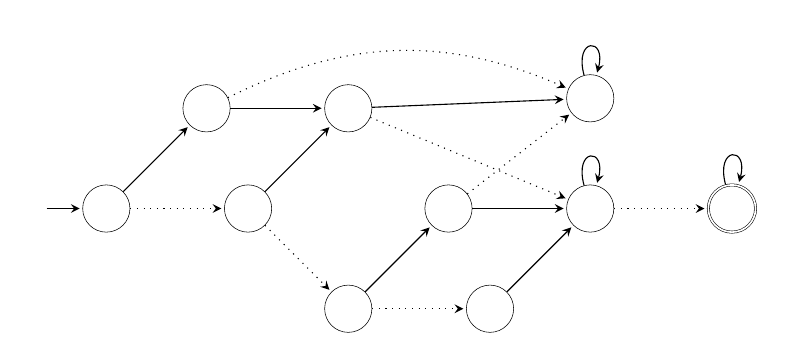
\begin{tikzpicture}[->,>=stealth,shorten >=1pt,auto,node distance=1.8cm,
        state/.style={circle,minimum size=6mm, very thin,draw=black,initial text=}]
        \node[state,initial] (0) {};
        \node[state] (1) [above right of=0] {};
        \node[state] (2) [right of=0] {};
        \node[state] (3) [right of=1] {};
        \node[state] (5) [below right of=2] {};
        \node[state] (6) [above right of=5] {};
        \node[state] (7) [right of=5] {};
        \node[state] (8) [right of=6] {};
        \node[state] (4) [above of=8,node distance=1.4cm] {};
        \node[state,accepting] (9) [right of=8] {};
        \path
          (0) edge node {} (1)
          (1) edge node {} (3)
          (2) edge node {} (3)
          (3) edge node {} (4)
          (4) edge[loop above] node {} (4)
          (5) edge node {} (6)
          (6) edge node {} (8)
          (8) edge[loop above] node {} (8)
          (7) edge node {} (8)
          (9) edge[loop above] node {} (9)
          (0) edge[dotted] node {} (2)
          (1) edge[bend left=25,dotted] node {} (4)
          (2) edge[dotted] node {} (5)
          (3) edge[dotted] node {} (8)
          (5) edge[dotted] node {} (7)
          (6) edge[dotted] node {} (4)
          (8) edge[dotted] node {} (9) ;
      \end{tikzpicture}
      \caption{There are three trees, namely , , and ; -transitions are dotted.}
      \label{fig:trees}
    \end{figure}
    Let  be the depth of , and let .
    If , then . 
    If , then .
    In both cases, .
    Now  is a disjoint union of such . 
    By the assumption, all trees are of depth at most ;
    recall that there is no -transition from  to~.
    Hence  follows.
  \qed
  \end{proof}

  The following lemma shows the lower bound 
  on the state complexity of the reverse of binary \R-trivial regular languages.

  \begin{lemma}\label{le:binaryRtriv_lower}
    For every ,
    there exists a binary \R-trivial regular language  with 
    such that .
  \end{lemma}
  \begin{proof}
    \begin{figure}[t]
      \centering
      \begin{tikzpicture}[->,>=stealth,shorten >=1pt,auto,node distance=1.8cm,
        state/.style={ellipse,minimum size=6mm,very thin,draw=black,initial text=}]
        \node[state,accepting] (0) {};
        \node[state] (1) [right of=0] {};
        \node[state] (2) [right of=1] {};
        \node[     ] (4) [right of=2] {};
        \node[state,initial right] (5) [right of=4] {};
        \node[state] (d) [left of=0] {};
        \path
          (0) edge[loop above] node {} (0)
          (d) edge[loop above] node {} (d)
          (1) edge node[above] {} (0)
          (1) edge[bend left=45] node[above] {\quad\,} (d)
          (2) edge node[above] {} (1)
          (5) edge node[above] {} (4)
          (4) edge node[above] {} (2) ;
      \end{tikzpicture}
      \caption{A binary \R-trivial regular language meeting the bound  for the reverse.}
      \label{fi:binaryRtriv}
    \end{figure}
    Consider the language 
    accepted by the partially ordered binary \mbox{-state} DFA 
    depicted in Fig.~\ref{fi:binaryRtriv}.
    We show that 
    each subset of  containing 
    is reachable in the subset automaton of the NFA .
    The proof is by induction on the size of subsets.
    The subset  is the initial state of the subset automaton.
    Each subset  of size  
    with 
    is reached from the subset  of size 
    by the string . 
  \qed
  \end{proof}

  Using a computer program 
  we have computed a few tight bounds 
  summarized in Table~\ref{tab}.
  The bound  is met by a DFA for  with  if ,
  but not if . 
  In addition, more than  states are reachable if ,
  but not if .
  By Lemma~\ref{lem:complement}, this means that for , the worst-case minimal partially ordered DFA has a dead state and so does its complement.
  It is worth mentioning that the witness languages are even \J-trivial, hence these tight upper bounds also apply to binary \J-trivial regular languages discussed in the next section.
  \begin{table}[h]
    \centering
      \begin{tabular}{c|c|c||c|c|l}
                     & \multicolumn{2}{c||}{Worst-case } &  &  & \\
                     & \multicolumn{2}{c||}{where DFA for  is}  &  &  & \\
                 & without    & with                           & Upper bound   & Lower bound & \\
             & dead state & dead state                     &  &    & \multicolumn{1}{c}{Witness}\\
        \hline
        1 & 1        & 1        & 1/2       & 1/2     & \\
        2 & 2        & 2        & 2         & 1       &  \\
        3 & 4        & 4        & 4         & 2       &  \\
        4 & 7        & 7        & 7         & 4       &  \\
        5 & 12       & 12       & 12        & 8       &  \\
        6 & 21       & 21       & 21        & 16      &  \\
        7 & {\bf 34} & 34       & {\bf 38}  & 32      &  \\
        8 & 55       & {\bf 64} & 71        & {\bf 64}&
      \end{tabular}
      \smallskip
      \caption{Tight bounds for the reverse of binary \R-trivial regular languages.}
      \label{tab}
  \end{table}
  
  We now prove that for , the upper bound is  for binary languages. 

  \begin{lemma}\label{lem:eight}
    Let  and let  be a binary \R-trivial regular language with .
    Then  and the bound is tight.
  \end{lemma}
  \begin{proof}
    Consider a minimal partially ordered -state DFA 
    over a binary alphabet .
    By definition, each maximal state of  has self-loops under both letters  and , hence there are at most two nonequivalent maximal states in .
    
    If there are two maximal states,
    then one of them is accepting and the other one is the dead state.
    The accepting state appears in all reachable subsets
    of the subset automaton of the NFA ,
    while the dead state appears in no reachable subset.
    Hence the number of reachable subsets is bounded by .
    
    It remains to prove that  is also the bound for  with only one maximal state.
    If the only maximal state is the dead state, we take the complement that has the same state complexity by Lemma~\ref{lem:complement}
    and has no dead state. 
    Thus, assume that  has a single maximal state, , which is accepting.
    Note that if a minimal binary partially ordered DFA has at least four states,
    there is a path of length two in the automaton.
    Consider three last states of such a longest path, say .
    In particular, there is no longer path from  to .  
    Note also that  is not accepting, otherwise it is equivalent to .
    As in the proof of Lemma~\ref{lem:binaryRtriv_upper},
    we can show that to reach the upper bound,
    the situation between states  and  must be as depicted in Fig.~\ref{fig:bound4}.
    \begin{figure}[t]
      \centering
      \begin{tikzpicture}[->,>=stealth,shorten >=1pt,auto,node distance=3.2cm,
        state/.style={ellipse,minimum size=6mm, very thin,draw=black,initial text=}]
        \node[state,accepting] (1) {};
        \node[state] (2) [left of=1] {};
        \node[state] (3) [left of=2] {};
        \path
          (1) edge[loop above] node {} (1)
          (2) edge node[above] {} (1)
          (2) edge[loop above] node {} (2)
          (3) edge node[above] {} (2);
      \end{tikzpicture}
      \caption{Path of length two, where .}
      \label{fig:bound4}
    \end{figure}
    
    We now compute the number of reachable sets in the subset automaton of the NFA 
    containing  and , but not .
    Recall from the proof of Lemma~\ref{lem:binaryRtriv_upper} that , ,
    reaches at most  different subsets. 

    If both  go from state  to state ,
    then there are at most  subsets in the subset automaton of the NFA  containing  and  and not ,
    namely  with .
    
    If , cf. Fig.~\ref{fig:bound4}, we have the following cases:
    (i)  goes to ,
    (ii)  goes to another state  (the case  is discussed above), or
    (iii)  is a self-loop in .

    In the first case, there is no subset containing  and  and not  reachable in the subset automaton of  
    because  is introduced by , which also introduces .

    In the second case, 
     must go to  (and only to  or ) 
    because  has only one maximal state, , and there is no longer path from  to .
    If  goes to  under ,
    then  appears in all subsets containing  and , 
    hence only  contains  and  and not .
    If  goes to  under  and  is a self-loop in ,
    then there are at most  subsets containing  and  and not , namely  with ,
    computed similarly as in the proof of Lemma~\ref{lem:binaryRtriv_upper}.
    If  goes to  under  and  is a self-loop in , then  is equivalent to  (if  is non-accepting) or to  (if  is accepting), hence it is not possible.


    In the third case,
    all subsets reachable in the subset automaton of  containing  and  and not  are  with . There are at most  such subsets (at most  nonempty subsets  in this case).


    If , we have the following cases:
    (i)  goes to ,
    (ii)  goes to another state , or
    (iii)  is a self-loop in .

    In the first case, there at most  subsets containing  and  and not , namely  with .

    In the second case,
     must again go to  (and only to  or ) for the same reason as above.
    If  goes to  under ,
    then  appears in all subsets containing  and , 
    hence at most  subsets,  with , contain  and  and not .
    If  goes to  under  and  is a self-loop in ,
    then there are at most  subsets containing  and  and not ,
    namely  subsets  and  subsets  with .
    If  goes to  under  and  is a self-loop in ,
    then  is equivalent to  (or to , see above).


    In the third case, all subsets containing  and  and not  are reachable only by strings with one , i.e., the reachable subsets are  with . Their number is at most  (at most  subsets  in this case).


    By the proof of Lemma~\ref{lem:binaryRtriv_upper}, there are at most  reachable sets in the subset automaton of  containing  and , and at most  reachable states not containing . Thus, for  and  with no dead state, the subset automaton of  has at most  reachable states (those containing , those containing  and not , and those containing  and not , respectively),
    which is less than  for .
    For  is the bound given by computation (Table~\ref{tab}).
  \qed
  \end{proof}

  Denote by  the state complexity function of the reverse
  on binary \R-trivial regular languages over a -element alphabet defined by
  
  Using this notation, 
  we can summarize our results
  in the following theorem.

  \begin{theorem}\label{thm1}
    Let  and let  be the state complexity of
    the reverse
    on \R-trivial regular languages over a -element alphabet.
    Then
    
  \end{theorem}  
  \begin{proof}
    Since the reverse of every unary language is the same language,
    we have .
    The upper bounds on  are given by Lemmas~\ref{lem:binaryRtriv_upper} and~\ref{lem:eight} and by 
    our calculations in the case of .
    The lower bounds in the case of 
    also follow from the calculations,
    while the case of  is covered by Lemma~\ref{le:binaryRtriv_lower}.
    The result for  is from Corollary~\ref{cor:bound}.
    Since adding  new letters to the ternary witness automata does not change
    the proofs  of reachability and distinguishability
    in the ternary case,
    the upper bound is tight for every .
  \qed
  \end{proof}


\section{\J-trivial regular languages}\label{***Jtriv}
  Every \J-trivial regular language is also \R-trivial, hence the previous bounds apply. To prove the results of this section, we first define {\em Simon's condition\/} on \R-trivial regular languages to be \J-trivial. 
  
  Let  be a DFA. It can be turned into a directed graph  with the set of vertices , where a pair  is an edge in  if there is a transition from  to  in . For , we define the directed graph  with the set of vertices  by considering only those transitions that correspond to letters in .
  
  For a directed graph  and , the set 
  
  is called the component of .

  \begin{definition}[Simon's condition]
    A DFA  with an input alphabet 
    satisfies Simon's condition
    if, for every subset  of , each component of  has a unique maximal state.
  \end{definition}

  Simon~\cite{Simon1975} has shown the following result.
  \begin{fact}\label{st}\label{fact:simon}
    An \R-trivial regular language is \J-trivial if and only if its minimal partially ordered DFA satisfies Simon's condition.
  \end{fact}

  Note that it is more efficient to use Trahtman's condition to decide whether an \R-trivial regular language is \J-trivial. For a state , let  denote the set of letters under which there is a self-loop in . Trahtman has shown that an \R-trivial regular language is \J-trivial if and only if its minimal partially ordered DFA satisfies that, for every state , the connected component of  containing  has a unique maximal state, see~\cite{Trahtman2001} for more details.
  
  Using Simon's result we immediately obtain the following lemma.
  \begin{lemma}\label{lem:removing}
    Let  .
    If a partially ordered DFA  over  satisfies Simon's condition, 
    then the DFA  (not necessarily connected) obtained from 
    by removing transitions under letters from 
    also satisfies Simon's condition.
  \end{lemma}
  \begin{proof}
    Let .
    By Fact~\ref{fact:simon}, each component of  has a unique maximal state and remains partially ordered.
    \qed
  \end{proof}

  We now prove the main result of this section.
  \begin{theorem}\label{thm:boundJtriv}
    At least  letters are necessary for a \J-trivial regular language of the state complexity  to reach the state complexity  in the reverse.
  \end{theorem}
  \begin{proof}
    We prove by induction on the number of states
    that every partially ordered DFA  satisfying Simon's condition with  states and at most  letters
    has less than  subsets reachable in the subset automaton of . 
 
    The basis for  holds since the automaton is over a unary alphabet, 
which means that the set  has at most three elements (cf. the proof of Lemma~\ref{lem:binaryRtriv_upper}).
    
    Assume that for some  the claim holds for every partially ordered DFA satisfying Simon's condition with at most  states and  letters. Let  be a partially ordered DFA satisfying Simon's condition with  states and  letters. We prove that less than  subsets are reachable in the subset automaton of the NFA . To do this, we show that reachability of  subsets in the subset automaton of  implies the existence of a partially ordered DFA  satisfying Simon's condition with  letters,  states and  reachable subsets in the subset automaton of the NFA . However, by the induction hypothesis, the number of reachable subsets in the subset automaton of  is less than , which means that the assumption of  reachable subsets in the subset automaton of  cannot hold.
    
    We may assume that  is connected and has no equivalent states, since any two equivalent states of  appear in the same sets in the subset automaton of , which implies reachability of less than  subsets in the subset automaton of . Similarly for two or more connected components. We may also assume that the unique maximal state of , denoted by , is accepting. Indeed, a subset  is reachable in the subset automaton of the reverse of  if and only if the set  is reachable in the subset automaton of the reverse of the complement of .
    
    To construct , we first define nonempty sets  and  such that  and use them to construct the (not necessarily connected) partially ordered DFA  from  by removing state  and all transitions labeled by letters from  and joining all states of  into a single state. We show that  satisfies Simon's condition and that it has  reachable subsets in the subset automaton of the reverse. Since  and , we obtain that  and induction applies.
    
    To construct the sets  and , 
    let  denote the set of all states different from  with a transition to ,
    and let  denote the set of letters connecting states of  with state .
    Note that  and  are nonempty.
    Let  be the -state subautomaton of  obtained by removing state 
    and all transitions labeled by letters from .
    By Lemma~\ref{lem:removing},  satisfies Simon's condition.
    
    Let  denote the set of states of  that are maximal in .
    For a state  in , let  denote the connected component of  containing ,
    and let  denote the set of labels connecting  to , see Fig.~\ref{fig:tree} for illustration.
    \begin{figure}[t]
      \tikzset{ 
        treenode/.style = {align=center, inner sep=0pt}, 
        ac/.style = {treenode, circle, black, draw=red,   text width=1.5em, very thick}, 
        na/.style = {treenode, circle, black,   draw=green, text width=1.5em, very thick} 
      }
      \centering
      \begin{tikzpicture}[-,>=stealth',level/.style={sibling distance = 5cm/#1, level distance = 1.3cm}]
        \node [ac] (1) {}
          child{ node [na] (2) {} edge from parent node[above left]  {} }
          child{ node [na] (3) {} edge from parent node[above right] {} } ;
        \path
          (1) edge[loop above] node {} (1)
          (2) edge[loop above] node {} (2)
          (3) edge[loop above] node {} (3);
        \draw (-2.5,-2) ellipse (1cm and 1.5cm);
        \draw (-2.5,-2.9) node {};
        \draw (2.5,-2) ellipse (1cm and 1.5cm);
        \draw (2.5,-2.9) node {};
      \end{tikzpicture}
      \caption{The partially ordered DFA ; .}
      \label{fig:tree}
    \end{figure}
    Note that  and  are not connected, for , otherwise  and  are two maximal states of the connected component containing . Next, we show that for every letter  in , there exists a state  in  such that  goes to  under .
    Let  be a letter from  and let  be a state in  with an -transition to  such that no other state reachable from  in  goes to  under . If  is not in , there is a state  in  such that  belongs to . But then there are two maximal states in the component containing  in the graph , namely  and the one reachable from  by letters from . Thus, .
Note that all states of  are non-accepting; if a state  of  is accepting, then, by the assumption, subset  is reachable in the subset automaton of . This requires to eliminate state  from the initial state . However, it can be done only by a letter from , which always introduces another state from .
    
    We now prove that , i.e., for every state  in ,
    there exists a letter  in 
    that does not appear in  for any other state  in .
    For the sake of contradiction,
    assume that there is a state  in  with .
Since all subsets containing  and  and not any  from 
    different from  are reachable in the subset automaton of ,
    state  is introduced to the subset from 
    by a transition under a letter from 
    which also introduces a state  into that subset.
    Since , 
    any attempt to eliminate state  results in the introduction of a state  different from , which is a contradiction.




    Let . Then  as required.
    Recall that the states of  are maximal in  and non-accepting.
    Thus, they do not appear in any reachable subset of the subset automaton of the reverse of .
Construct the DFA  from 
    by joining all states of  into one state.
    Then the subset automaton of the reverse of 
    has the same number of reachable subsets
    as the subset automaton of the reverse of ,
    and  satisfies Simon's condition.

    Finally, we show that  (hence also ) has  reachable subsets in the subset automaton of the reverse.
    Since  is accepting, each set  containing  and nothing from  is reachable in the subset automaton of  only by symbols from  (otherwise a symbol from  is introduced and we cannot get rid of states of  anymore),
    hence the set  is reachable in the subset automaton of .
As there are  such sets,  has  reachable subsets in the subset automaton of the reverse.
    This leads to the contradiction explained above and completes the proof.
  \qed\end{proof}
  
  Using this result, we can prove the tight upper bound 
  on the state complexity of the reverse 
  for \J-trivial regular languages over an -element alphabet.

  \begin{theorem}\label{thm3}
    Let  and let  be a \J-trivial regular language
    over an -element alphabet with  .
    Then  and the bound is tight.
  \end{theorem}
  \begin{proof}
    The upper bound follows from Theorem~\ref{thm:boundJtriv}.
    \begin{figure}[t]
      \centering
      \begin{tikzpicture}[->,>=stealth,shorten >=1pt,auto,node distance=2.4cm,
        state/.style={ellipse,minimum size=6mm, very thin,draw=black,initial text=}]
        \node[state,initial] (2) {};
        \node[state] (3) [right of=2] {};
        \node[     ] (4) [right of=3] {};
        \node[state] (5) [right of=4] {};
        \node[state] (6) [right of=5] {};
        \node[state,accepting] (d) [below right of=3] {};
        \path
          (2) edge node {} (3)
          (3) edge node {} (d)
          (3) edge node {} (4)
          (4) edge node {} (5)
          (5) edge[loop above] node {} (5)
          (5) edge node[above left] {} (d)
          (5) edge node {} (6)
          (6) edge[loop above] node {} (6)
          (6) edge[bend left=20] node[above left] {} (d)
          (d) edge[loop above] node {} (d) ;
      \end{tikzpicture}
      \caption{The witness minimal partially ordered DFA  satisfying Simon's condition.}
      \label{fig:n2witness}
    \end{figure}
    Thus, to prove tightness, we consider 
    the \J-trivial regular language accepted by the minimal DFA 
    
    depicted in Fig.~\ref{fig:n2witness}.
    The transitions under a letter  in  are defined by
    
    The initial state of the subset automaton of the NFA  is the set  and, for , 
    every -element set  
    with  
    is reached from the -element set  by .
    This gives  reachable states (those containing 0 and not 1).
    Note that the set  is not reachable,
    but all subsets of the state set of  of cardinality at least three containing  and 
    are reachable
    since every set  is reached from the set
     by letter .
    \qed
  \end{proof}

  Lemma~\ref{lem:eight} also gives the upper bound for binary \J-trivial regular languages. The witness languages in Table~\ref{tab} are \J-trivial. For , we need a dead state to reach the upper bound  and our witness automata have a dead state (Fig.~\ref{fi:binaryRtriv}), hence the language is not \J-trivial.
  \begin{corollary}
    Let  be a binary \J-trivial regular language with , 
    where , then . 
    A few tight upper bounds for  are given in Table~\ref{tab}.
    \qed
  \end{corollary}
  
  Concerning the lower bound state complexity, it was shown in~\cite{CampeanuCSY99} that there are finite binary languages whose reverse have a blow-up of , for  even, and of , for  odd. Since every finite language is \J-trivial, we obtain at least these lower bounds for binary \J-trivial regular languages.

\section{Conclusions}\label{***conclu}
  We have presented a characterization of tight bounds on the state complexity of the reverse for \R-trivial regular languages depending not only on the state complexity of the language, but also on the size of its alphabet. As a consequence, this characterization also gives upper bounds for \J-trivial regular languages, but they are not reachable for languages of the state complexity  over an -element alphabet, for . We have further shown tight bounds for \J-trivial regular languages over - and -element alphabets, but (except for a few examples for binary \J-trivial regular languages) the problem of the tight bounds for \J-trivial regular languages over an alphabet of a lower cardinality is open.

\subsubsection*{Acknowledgements.}
  The authors gratefully acknowledge comments and suggestions of anonymous referees.

\bibliographystyle{splncs}
\bibliography{dcfs2013}

\end{document}
